\documentclass[10pt]{beamer}

\usetheme[progressbar=frametitle]{metropolis}
\usepackage{appendixnumberbeamer}

\usepackage{booktabs}

% % For removing Figure 1 in figures
\usepackage{caption}

%For linking email and website
\usepackage{hyperref}

%For enumeration as words
\usepackage{blindtext}
\usepackage{enumitem}
\usepackage{geometry}

\usepackage{tikz}
\usepackage{xspace}


\title{Theory of Computation}
\subtitle{Tutorial - Math Preliminaries}
\author{Cesare Spinoso-Di Piano}
\date{}

\begin{document}

\maketitle

\begin{frame}{Plan for today}
    \setbeamertemplate{section in toc}[sections numbered]
    \tableofcontents[hideallsubsections]
\end{frame}

\section{Introduction}


\begin{frame}{Expectations}
    \begin{itemize}
        \item[-] This is yet another theoretical computer science resource to study from.
        \item[-] PDFs of these slides and additional notes/exercises on my website \href{https://cesare-spinoso.github.io/teaching/theoretical_cs}{https://cesare-spinoso.github.io/teaching/theoretical\_cs}
        \item[-] Some exercises will have typed solutions and others will have video solutions (and others might just have no solutions).
        \item[-] If there's anything you think could be added or improved, don't hesitate to let me know (submit an issue on GitHub).
    \end{itemize}
\end{frame}

\section{Review of set theory}

\begin{frame}{Definition of a set}
    \textbf{Definition.} A set $S$ is an unordered, well-defined collection of distinct elements.
    \begin{itemize}
        \item \textbf{Example 1.} $S_1 = \{1,2,8,twenty,\#,**,56 \}$ - \textit{Finite} set.
        \item \textbf{Example 2.} $S_2 = \{1,2,3,...,49\}$.
        \item \textbf{Example 3.} $S_2 = \{n: \text{n is an integer greater than 23}\}$.
        \item \textbf{Example 4.} $S_3 = \{n \in \mathbb{Z}:n \geq 0 \And n=2k \}$ - \textit{Infinite} set of ...?
        \item \textbf{Example 5.} What do the sets $\mathbb{N},\mathbb{Z}, \mathbb{Q}$ and $\mathbb{R}$ represent?
        \item \textbf{Example 6.} $S_4 = \{n^3 - 3: n \in \mathbb{Z} \And 0 \leq n \leq 27 \}$ - What's the smallest number in this set? Is it finite or infinite?
    \end{itemize}
    Examples 1 and 2 use an explicit notation. Example 3 uses natural language. Example 4 and 6 use set builder notation.
\end{frame}

\begin{frame}{Membership}
    If an element $a$ belongs to a set $A$, write $a \in A$. Otherwise, $a \notin A$.
    \begin{itemize}
        \item \textbf{Example 1.} $A_1 = \{1,2,3,...,75 \}$ Does $2 \in A_1$? Does $-45 \in A_1$?
        \item \textbf{Example 2.} $A_2 = \{m^2 + 1: m \in \mathbb{Z}  \}$
              \begin{itemize}
                  \item \textbf{1.} Does $2 \in A_2$?
                  \item \textbf{2.} $65 \in A_2$?
                  \item \textbf{3.} $-17 \in A_2$?
                  \item \textbf{4.} $49 \in A_2$?
                  \item Would any of the answers be different if $m \in \mathbb{R}$?
              \end{itemize}
    \end{itemize}
\end{frame}

\begin{frame}{Subset}
    \textbf{Definition.} A set $A$ is a \textit{subset} of $B$ if every element in $A$ is also in $B$. We write $A \subseteq B$.
    \begin{itemize}
        \item \textbf{Example 1.} $\{1,3,4,5\} \subseteq \{1,3,4,5\}$
        \item \textbf{Example 2.} Is it true that $\mathbb{N} \subseteq \mathbb{Z}$? What about $\mathbb{R} \subseteq \mathbb{Z}$? Why or why not?
    \end{itemize}

    \textbf{Definition.} A set $A$ is a \textit{proper subset} of $B$ if every element in $A$ is also in $B$ AND $A \neq B$. We write $A \subset B$.
    \begin{itemize}
        \item \textbf{Example 1.} $\{1,3,5\} \subset \{1,3,4,5\}$. Would $\subseteq$ also be correct?
        \item \textbf{Example 2.} Does $A \subseteq B$ imply $A \subset B$? What about the other way? Can you find examples or sketch a proof?
    \end{itemize}
\end{frame}

\begin{frame}{Empty Set}
    \textbf{Definition.} The empty set denoted as $\varnothing, \emptyset, \{\}$ is the set that does not contain any elements. It is NOT nothing!\\
    \begin{itemize}
        \item \textbf{Example 1.} $\{n:n\geq 0 \And n < 0\}$.
        \item \textbf{Example 2.} $\{n:n \in \mathbb{Z} \And n^2 = -1 \}$
        \item \textbf{Example 3.} True or False: The empty set is a subset of any set.
    \end{itemize}
\end{frame}

\begin{frame}{Universal set}

    \textbf{Definition.} The universal set denoted $U$ is the set that contains ALL elements (in the context of the problem). The universal set is usually defined at the beginning or implied.
    \begin{itemize}
        \item \textbf{Example 1.} If $S=\{2k:k\in \mathbb{Z}\}$ then an appropriate universal set would be $U=\mathbb{Z}$.
    \end{itemize}

\end{frame}

\begin{frame}{Power sets}
    \textbf{Definition.} Given a set $S$, its power set $2^S$ or $\mathcal{P}(S)$ is the set of ALL subsets of $S$. This means that all the elements in $2^S$ are \underline{sets}.
    \begin{itemize}
        \item \textbf{Example 1.} What is the power set of $\{a,b,c\}$?
        \item \textbf{Example 2.} What is the power set of $\emptyset$?
        \item \textbf{Example 3.} Give an example of a set $S$ for which $\mathcal{P}(S) = S$?
    \end{itemize}
\end{frame}

\begin{frame}{Cardinality}
    \textbf{Definition.} The cardinality of $S$ denoted $|S|$ is the number of elements in the set $S$.
    \begin{itemize}
        \item \textbf{Example 1.} For $S = \{1,2,3,4\}$, $|S| = 4$.
        \item \textbf{Example 2.} Given $S = \{1,2,\{1,2,\emptyset,\{\emptyset\}\},4 \}$, what is $|S|$?
        \item \textbf{Example 3.} If $S$ is \textit{finite}, what is $|2^S|$? That is for any finite set, what is the size of its power set?
    \end{itemize}
    If a set is \textit{infinite}, it is either countably infinite or uncountably infinite.
\end{frame}

\begin{frame}{Set operations - Union}
    \textbf{Definition.} Let $A$ and $B$ be two sets. The \textbf{union} of $A$ and $B$ is defined as $A \cup B = \{x:x \in A \text{\hspace{1mm}or\hspace{1mm}} x \in B \}$.
    \begin{itemize}
        \item \textbf{Example 1.} $A=\{1,2,3\}$ $B=\{2,3,4\}$. What is $A \cup B$?
        \item \textbf{Example 2.} If $U$ is the universal set and $S$ is some other set, what is $U \cup S$?
    \end{itemize}
\end{frame}

\begin{frame}{Set operations - Intersection}
    \textbf{Definition.} Let $A$ and $B$ be sets. The \textbf{intersection} of $A$ and $B$ is defined as $A \cap B = \{x: x \in A \And x \in B\}$.
    \begin{itemize}
        \item \textbf{Example 1.} $A=\{1,2,3\}$ $B=\{2,3,5,6\}$. What is $A \cap B$?
        \item \textbf{Example 2.} If $U$ is the universal set. What is $\emptyset \cap U$?
    \end{itemize}
\end{frame}

\begin{frame}{Set operations - Complement}
    \textbf{Definition.} Let $A$ be a set. The \textbf{complement} of $A$ is defined using $U$ as $\overline{A} = \{x: x \notin A \And x \in U\}$. (It is everything \textbf{not} in $A$).
    \begin{itemize}
        \item \textbf{Example 1.} $A = \{1,2,3\}$. What is $\overline{A}$. Yes, this is a trick question.
        \item \textbf{Example 2.} $A = \{1,2,3\}$ $U = \{x: 1 \leq x \leq 10, x \in \mathbb{Z}\}$. What is $\overline{A}$?
        \item \textbf{Example 3.} What is $\overline{\emptyset}$ and $\overline{U}$?
    \end{itemize}
\end{frame}

\begin{frame}{Set operations - Difference}
    \textbf{Definition.} Let $A$ and $B$ be sets. The \textbf{difference} of $A$ and $B$ is defined as $A - B = \{x: x \in A \And x \notin B\}$. (Everything in $A$ \textbf{not in} $B$).
    \begin{itemize}
        \item \textbf{Example 1.} $A = \{1,2,3,4,5\}$ $B=\{2,5,6,7\}$. What is $A - B$? $B - A$?
        \item \textbf{Example 2.} What is $A - \emptyset$? $\emptyset - A$? $P(\emptyset) - \emptyset$?
        \item \textbf{Example 3.} Rewrite $A - B$ using only the union ($\cup$), intersection ($\cap$) and complement ($-$) operator.
    \end{itemize}
\end{frame}

\begin{frame}{Set operations - Cross-product}
    \textbf{Definition.} The \textbf{cross-product} of $A$ and $B$ is defined as $A \times B = \{(a,b): a \in A \And b \in B\}$. It is a set of two-tuples.
    \begin{itemize}
        \item \textbf{Example 1.} $A = \{1,2,3\}$ $B = \{5,6\}$. What is $A \times B$?
        \item \textbf{Example 2.} What is $|A \times B|$?
        \item \textbf{Example 3.} What is $S \times \emptyset$?
    \end{itemize}
\end{frame}

\begin{frame}{Set operations - Exercises}
    Let $U = \{1,2,4,7,8,9,10,11\}, A = \{7,8,9\}, B = \{4,9,10\}$. What do the following set operations yield?
    \begin{itemize}
        \item \textbf{a.} $A \cup B = ...$
        \item \textbf{b.} $A \cap B = ...$
        \item \textbf{c.} $A - B = ...$
        \item \textbf{d.} $\overline{A} \cap B = ...$
        \item \textbf{e.} $A \times \{1,2\} = ...$
        \item \textbf{f.} $ (A \times B) \cap \emptyset = ...$
        \item \textbf{g.} $ (\overline{A} \cup \overline{B}) \cup U = ...$
        \item \textbf{h.} $U \times \emptyset = ...$
        \item \textbf{i.} $ (\overline{A} \cup \overline{\emptyset}) \cap U = ...$
    \end{itemize}
\end{frame}

\begin{frame}{Set operations - Some more properties}
    Given the set $S$, the following are always true:
    \begin{itemize}
        \item \textbf{1.} $S \cup U = U$
        \item \textbf{2.} $S \cap U = S$
        \item \textbf{3.} $S \cup \emptyset = S$
        \item \textbf{4.} $S \cap \emptyset = \emptyset$
        \item \textbf{5.} $S \times \emptyset = \emptyset$
        \item \textbf{6.} $\overline{\overline{S}} = S$
        \item \textbf{7.} $\overline{\emptyset} = U$
        \item \textbf{8.} $\overline{U} = \emptyset$
    \end{itemize}
    \textbf{Theorem (De Morgan's Law).} Given two sets $S_1$ and $S_2$:
    \begin{itemize}
        \item $\overline{S_1 \cap S_2} = \overline{S_1} \cup \overline{S_2}$
        \item $\overline{S_1 \cup S_2} = \overline{S_1} \cap \overline{S_2}$
    \end{itemize}
\end{frame}

\section{Review of graph theory}

\begin{frame}{Definition of a graph}
    \textbf{Definition.} An \textbf{undirected graph} is a collection of points (called \textbf{vertices/nodes}) with lines (called \textbf{edges}) connecting some of the points.

    In an undirected graph, there is no direction to the edges. In a directed graph, edges have have arrows to signal direction.


    \textbf{Example.} The following are two examples of graphs. $G_a$ is undirected, $G_b$ is directed.
    \begin{figure}
        \centering
        \hfill
        \begin{minipage}{0.3\textwidth}
            \centering
            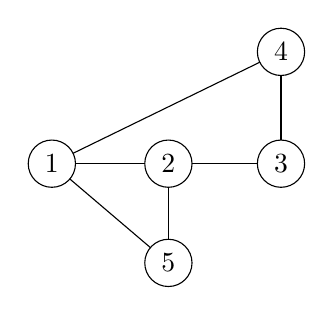
\begin{tikzpicture}[scale=0.1]
                \tikzstyle{every node}+=[inner sep=0pt]
                \draw [black] (32,-29.3) circle (3);
                \draw (32,-29.3) node {$1$};
                \draw [black] (46.8,-29.3) circle (3);
                \draw (46.8,-29.3) node {$2$};
                \draw [black] (61.1,-29.3) circle (3);
                \draw (61.1,-29.3) node {$3$};
                \draw [black] (61.1,-15.1) circle (3);
                \draw (61.1,-15.1) node {$4$};
                \draw [black] (46.8,-41.9) circle (3);
                \draw (46.8,-41.9) node {$5$};
                \draw [black] (34.28,-31.24) -- (44.52,-39.96);
                \draw [black] (35,-29.3) -- (43.8,-29.3);
                \draw [black] (49.8,-29.3) -- (58.1,-29.3);
                \draw [black] (46.8,-32.3) -- (46.8,-38.9);
                \draw [black] (58.4,-16.42) -- (34.7,-27.98);
                \draw [black] (61.1,-18.1) -- (61.1,-26.3);
            \end{tikzpicture}
            \caption*{Graph $G_a$}
        \end{minipage}\hfill\begin{minipage}{0.3\textwidth}
            \centering
            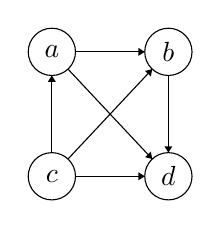
\begin{tikzpicture}[scale=0.1]
                \tikzstyle{every node}+=[inner sep=0pt]
                \draw [black] (32,-29.3) circle (3);
                \draw (32,-29.3) node {$a$};
                \draw [black] (46.8,-29.3) circle (3);
                \draw (46.8,-29.3) node {$b$};
                \draw [black] (46.8,-45.1) circle (3);
                \draw (46.8,-45.1) node {$d$};
                \draw [black] (32,-45.1) circle (3);
                \draw (32,-45.1) node {$c$};
                \draw [black] (35,-29.3) -- (43.8,-29.3);
                \fill [black] (43.8,-29.3) -- (43,-28.8) -- (43,-29.8);
                \draw [black] (46.8,-32.3) -- (46.8,-42.1);
                \fill [black] (46.8,-42.1) -- (47.3,-41.3) -- (46.3,-41.3);
                \draw [black] (32,-42.1) -- (32,-32.3);
                \fill [black] (32,-32.3) -- (31.5,-33.1) -- (32.5,-33.1);
                \draw [black] (35,-45.1) -- (43.8,-45.1);
                \fill [black] (43.8,-45.1) -- (43,-44.6) -- (43,-45.6);
                \draw [black] (34.05,-31.49) -- (44.75,-42.91);
                \fill [black] (44.75,-42.91) -- (44.57,-41.98) -- (43.84,-42.67);
                \draw [black] (34.05,-42.91) -- (44.75,-31.49);
                \fill [black] (44.75,-31.49) -- (43.84,-31.73) -- (44.57,-32.42);
            \end{tikzpicture}
            \caption*{Graph $G_b$}
        \end{minipage}
    \end{figure}
\end{frame}

\begin{frame}{Formal representation of a graph}
    A graph can be represented pictorially or more formally by a set of vertices $V$ and edges $E$.

    For \textbf{undirected graphs}, we write $G = (V, E)$ where $V$ is the set of vertices (more specifically their labels) and $E$ is the set of edges where an edge is itself represented as a set $\{a, b\}$ of vertices.

    For \textbf{directed graphs}, the notation is the same except that edges are represented by tuples $(a, b)$ to signal that the edge goes out of $a$ into $b$.

    \textbf{Example.} The graphs from the previous slide could have also been written as
    \begin{itemize}
        \item $G_a = (\{1, 2, 3, 4, 5\}, \{\{1, 4\}, \{1, 2\}, \{1, 5\}, \{2, 5\}, \{2, 3\}, \{3, 4\}\})$
        \item $G_b = (\{a, b, c, d\}, \{(a, b), (a, d), (b, d), (c, a), (c, b), (c, d)\})$
    \end{itemize}
\end{frame}

\begin{frame}{Ways of ``walking'' through a graph}
    There are several different ways to ``walk'' through a graph. Each way has its own name and characteristics.
    \begin{itemize}
        \item A \textbf{walk} from vertex $v_{i_1}$ to $v_{i_n}$ is a sequence of edges $(v_{i_1}, v_{i_2}), (v_{i_2}, v_{i_3}), \dots, (v_{i_{n-1}}, v_{i_n})$ where both vertices and edges may repeat. Notice that the sequence must be ``contiguous'' i.e. the edge $e_i$ in the sequence must start at the destination vertex of $e_{i-1}$.
        \item A \textbf{path} is a walk in which no edge is repeated.
        \item A \textbf{simple path} is a path in which no vertex is repeated.
    \end{itemize}
    \textbf{Example.} (Simple) Path $(1, 2), (2, 3), (3, 4)$
    \begin{figure}
        \centering
        \begin{minipage}{0.4\textwidth}
            \centering
            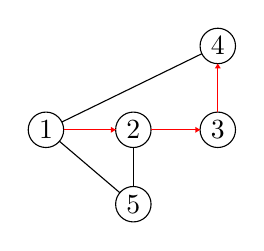
\begin{tikzpicture}[scale=0.075]
                \tikzstyle{every node}+=[inner sep=0pt]
                \draw [black] (32,-29.3) circle (3);
                \draw (32,-29.3) node {$1$};
                \draw [black] (46.8,-29.3) circle (3);
                \draw (46.8,-29.3) node {$2$};
                \draw [black] (61.1,-29.3) circle (3);
                \draw (61.1,-29.3) node {$3$};
                \draw [black] (61.1,-15.1) circle (3);
                \draw (61.1,-15.1) node {$4$};
                \draw [black] (46.8,-41.9) circle (3);
                \draw (46.8,-41.9) node {$5$};
                \draw [black] (34.28,-31.24) -- (44.52,-39.96);
                \draw [red] (35,-29.3) -- (43.8,-29.3);
                \fill [red] (43.8,-29.3) -- (43,-28.8) -- (43,-29.8);
                \draw [red] (49.8,-29.3) -- (58.1,-29.3);
                \fill [red] (58.1,-29.3) -- (57.3,-28.8) -- (57.3,-29.8);
                \draw [black] (46.8,-32.3) -- (46.8,-38.9);
                \draw [black] (58.4,-16.42) -- (34.7,-27.98);
                \draw [red] (61.1,-18.1) -- (61.1,-26.3);
                \fill [red] (61.1,-18.1) -- (60.6, -18.9) -- (61.6, -18.9);
            \end{tikzpicture}
        \end{minipage}\hfill
    \end{figure}
\end{frame}

\begin{frame}{Ways of ``looping'' through a graph}
    There are also different ways to ``loop'' through a graph i.e. starting and ending at the same vertex.
    \begin{itemize}
        \item A \textbf{self-loop} or just \textbf{loop} is an edge that starts and ends at the same vertex. That is, its \textbf{outgoing} and \textbf{incoming} vertices are the same.
        \item A \textbf{circuit} with base $v_i$ is a walk that starts and ends at $v_i$.
        \item A \textbf{cycle} is a circuit with no repeated edges.
        \item A \textbf{simple cycle} is a cycle with no repeated vertices other than its first vertex.
    \end{itemize}
    \textbf{Example.} (Simple) Cycle with base $a$, $(a, d), (d, c), (c, a)$
    \begin{figure}
        \begin{minipage}{0.3\textwidth}
            \centering
            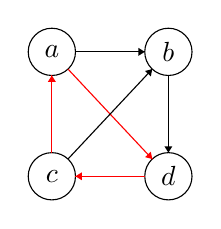
\begin{tikzpicture}[scale=0.1]
                \tikzstyle{every node}+=[inner sep=0pt]
                \draw [black] (32,-29.3) circle (3);
                \draw (32,-29.3) node {$a$};
                \draw [black] (46.8,-29.3) circle (3);
                \draw (46.8,-29.3) node {$b$};
                \draw [black] (46.8,-45.1) circle (3);
                \draw (46.8,-45.1) node {$d$};
                \draw [black] (32,-45.1) circle (3);
                \draw (32,-45.1) node {$c$};
                \draw [black] (35,-29.3) -- (43.8,-29.3);
                \fill [black] (43.8,-29.3) -- (43,-28.8) -- (43,-29.8);
                \draw [black] (46.8,-32.3) -- (46.8,-42.1);
                \fill [black] (46.8,-42.1) -- (47.3,-41.3) -- (46.3,-41.3);
                \draw [red] (32,-42.1) -- (32,-32.3);
                \fill [red] (32,-32.3) -- (31.5,-33.1) -- (32.5,-33.1);
                \draw [red] (35,-45.1) -- (43.8,-45.1);
                \fill [red] (35,-45.1) -- (35.8,-44.6) -- (35.8,-45.6);
                \draw [red] (34.05,-31.49) -- (44.75,-42.91);
                \fill [red] (44.75,-42.91) -- (44.57,-41.98) -- (43.84,-42.67);
                \draw [black] (34.05,-42.91) -- (44.75,-31.49);
                \fill [black] (44.75,-31.49) -- (43.84,-31.73) -- (44.57,-32.42);
            \end{tikzpicture}
        \end{minipage}
    \end{figure}
\end{frame}

\begin{frame}{Trees!}
    \textbf{Definition.} A graph $G=(V, E)$ is \textbf{connected} if for every pair of vertices $u, v \in V$ there is a path from $u$ to $v$.

    \textbf{Definition.} A \textbf{tree} is a connected acyclic graph. That is a connected graph with no cycles in it.

    \textbf{Definition.} A \textbf{forest} is a (not necessarily connected) acyclic graph. A forest is usually thought of as a collected of unconnected trees.

    \textbf{Definition.} A \textbf{rooted tree} is a directed tree that has one special vertex called the \textbf{root}. For every other vertex in the tree there exists a unique directed path to it from the root.

    \textbf{Example.} Removing edges $\{1,4\}$ and $\{1,5\}$ from graph $G_a$ makes it a tree

    \begin{figure}
        \centering
        \vspace{-5mm}
        \begin{minipage}{0.4\textwidth}
            \centering
            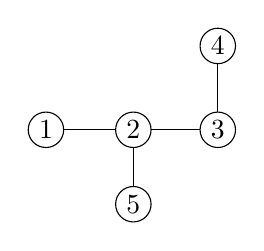
\begin{tikzpicture}[scale=0.075]
                \tikzstyle{every node}+=[inner sep=0pt]
                \draw [black] (32,-29.3) circle (3);
                \draw (32,-29.3) node {$1$};
                \draw [black] (46.8,-29.3) circle (3);
                \draw (46.8,-29.3) node {$2$};
                \draw [black] (61.1,-29.3) circle (3);
                \draw (61.1,-29.3) node {$3$};
                \draw [black] (61.1,-15.1) circle (3);
                \draw (61.1,-15.1) node {$4$};
                \draw [black] (46.8,-41.9) circle (3);
                \draw (46.8,-41.9) node {$5$};
                \draw [black] (35,-29.3) -- (43.8,-29.3);
                \draw [black] (49.8,-29.3) -- (58.1,-29.3);
                \draw [black] (46.8,-32.3) -- (46.8,-38.9);
                \draw [black] (61.1,-18.1) -- (61.1,-26.3);
            \end{tikzpicture}
        \end{minipage}\hfill
    \end{figure}
\end{frame}

\section{Review of (some) proof techniques}

\begin{frame}{Equality of sets}
    \textbf{Proof Technique.} To prove for two sets $A, B$ that $A = B$, one way of doing this is by ``double inclusion'' where you first show that $A \subseteq B$ and then $B \subseteq A$. To show that $A \subseteq B$, you must pick an \underline{arbitrary} element $a \in A$ (i.e. an element for which you only know about its belonging to $A$) and show that it is is $B$.
\end{frame}

\begin{frame}[t]{Example}
    \textbf{Example.} Prove that $\overline{A \cap B} = \overline{A} \cup \overline{B}$.
\end{frame}

\begin{frame}{Pigeonhole Principle}
    \textbf{Proof Technique.} The Pigeonhole Principle states that if there are $n+1$ pigeons occupying $n$ holes, there must be a hole with two pigeons.
\end{frame}

\begin{frame}[t]{Example}
    \textbf{Example.} Let $G = (V, E)$ be a simple graph, if $|V| \geq 2$ there exists two vertices $u, v \in V$ with the same degree.
\end{frame}

\begin{frame}{Proof by contradiction}
    \textbf{Proof Technique.} In a proof by contradiction, you assume that the premise of the statement you're trying to prove is false i.e. in if $P$ then $Q$ assume $P$ is false. You then reason through a sequence of steps to arrive to a contradiction which may be 1. a refutation of what you initially assumed or 2. a refutation of something you know/have proved to be true.
\end{frame}

\begin{frame}[t]{Example}
    \textbf{Example.} If $T = (V, E)$ is a tree, then for any two vertices $u, v \in V$ there exists a unique path between them.
\end{frame}

\begin{frame}{Proof by induction}
    \textbf{Proof Technique.} In a proof by induction, you want to prove a statement, $P(n)$, that depends on some integer $n$. For example, $P(n): $ ``For $n \geq 5$, $2^n \geq n^2$''. To do so, you must reason sequentially as follow
    \begin{itemize}
        \item[1.] Prove the \textbf{base case (BC)} $\rightarrow$ show that $P(n)$ is true for the smallest possible value of $n$.
        \item[2.] Assume the \textbf{inductive hypothesis} $\rightarrow$ assume that $P(n)$ is true for some arbitrary $n$.
        \item[3.] Prove the \textbf{inductive step} $\rightarrow$ show that $P(n+1)$ is true.
    \end{itemize}
\end{frame}

\begin{frame}[t]{Example}
    \textbf{Example.} Let $T = (V, E)$ be a tree. Prove that $|E| = |V| - 1$.
\end{frame}


\begin{frame}{Proof by construction}
    \textbf{Proof Technique.} In statements that claim the existence of some property or object, one common approach is to construct this property or object in the proof. This proof technique will be \underline{very common} in automata theory as you will see shortly.
\end{frame}

\begin{frame}[t]{Example}
    \textbf{Example.} (Sipser 0.10) For each even number $n$ greater than 2, there exists a 3-regular graph with $n$ vertices.
\end{frame}

\end{document}